\section{1174087 - Ilham Muhammad Ariq}
\subsection{Teori}
\begin{enumerate}
	\item Definisi Kecerdasan Buatan
		\par Kecerdasan Buatan adalah suatu ilmu yang mempelajari bagaimana cara komputer melakukan sesuatu seperti yang dilakukan oleh manusia. Secara sederhana AI adalah teknik dan ilmu untuk membangun atau membuat suatu mesin menjadi cerdas, terutama pada program komputer. Kecerdasan yang dimaksud yaitu seperti yang dimiliki oleh manusia namun pada mesin akan dibuat cepat dan tepat atau akurat.

\item Sejarah Kecerdasan Buatan
	\par Sejarah kecerdasan buatan dimulai pada zaman kuno. Benih kecerdasan buatan modern ditanamkan oleh filusuf klasik dengan berusaha menggambarkan proses berpikir manusia. Karya tersebut memuncak pada penemuan komputer digital yang di program pada tahun 1940 an, dimana terdapat sebuah mesin yang didasarkan pada esensi abstrak penalaran matematika.Istilah kecerdasan buatan pertama kali dikemukaan pada tahun 1956 di Konferensi Darthmouth yang kemudian sejak saat itu kecerdasan buatan terus berkembang. Artificial intelligence merupakan inovasi baru di bidang ilmu pengetahuan yang terbentuk sejak adanya komputer modern sekitar tahun 1940 dan 1950. Ilmu pengetahuan komputer ini khusus ditujukan dalam perancangan otomatisasi tingkah laku cerdas dalam sistem kecerdasan komputer. Pada awal 50-an, studi tentang “mesin berpikir” memiliki berbagai nama seperti cybernetics, teori automata, dan pemrosesan innformasi. Pada tahun 1956, para ilmuan jenius seperti Alan Turing, Norbert, Wiener, Claude Shannon dan Warren McCullough telah bekerja secara independen dibidang cybernetics, matematika, algoritma dan teori jaringan. Namun, seorang ilmuan komputer dan kognitif John McCarthy adalah orang yang dating dengan ide untuk bergabung dengan upaya penelitian terpisah ini kedalam satu bidang yang akan mempelajari topic baru untuk imajinasi manusia yaitu kecerdasan buatan. Dia adalah orang yang menciptakan istilah tersebut dan kemudian mendirikan laboratorium Kecerdasan Buatan di MIT dan Stan ford. Pada tahun 1956, McCarthy yang sama mendirikan Konferensi Dartmouth di Hanover, New Hampshire. Peneliti terkemuka dalam teori kompleksitas, simulasi bahasa, hubungan antara keacakan dan pemikiran kreatif, jaringan saraf diundang. Tujuan dari bidang penelitian yang baru dibuat adalah untuk mengembangkan mesin yang dapat mensimulasikan setiap aspek kecerdasab. Itulah sebabnya Konferensi Dartmouth 1956 dianggap sebagai kelahiran Kecerdasan Buatan. Sejak saat itu, Kecerdasa Buatan telah hidup melalui decade kemuliaan dan cemoohan, yang dikenal luas sebagai musim panas dan musim dingin AI. Musim panasnya ditandai dengan optimis dan dana besar,sedangkan musim dinginnya dihadapkan dengan pemotongan dana, ketidakkpercayaan dan pesimisme.

\item Perkembangan kecerdasan buatan
	\par Teknologi Artificial Intelligence semakin ramai dibahas dalam berbagai diskusi teknologi di seluruh dunia. Menurut kebanyakan orang, pekerjaan seperti kasir, operator telepon, pengendara truk, dan lainnya sangat berpeluang besar untuk tergantikan oleh Artificial Intelligence. Mengapa demikian? dikarenakan memang bahwa AI lebih unggul dalam hal kinerja, fitur dan lain sebagainya. Namun, dalam beberapa aspek memang pekerja manusia masih unggul dibandingkan AI itu sendiri. Para SCIKIT-LEARN 3 generasi muda yang ada di dunia terutama di daerah Asia terlihat sudah memahami fungsi dan efek dari AI dalam kehidupan kita sehari-hari. Berdasarkan survei yang dilakukan oleh Microsoft, terdapat 39 persen responden yang mempertimbangkan untuk menggunakan mobil tanpa pengemudi dan 36 persen lainnya setuju bahwa robot masa depan dengan software untuk beroperasi mampu meningkatkan produktivitas. Dari survey tersebut kita sebagai pengguna AI harus lebih bijaksana dalam pengembangan dan penggunaan dari AI sehingga tanpa memberikan efek samping terhadap etos kerja dan keseharian kita sebagai pengguna dalam kehidupan seharihari. AI Summer 1 (1956-1973) KOnferensi Dartmounth diikuti oleh 17 tahun kemajuan luar biasa. Proyek penelitian yang dilakukan di MIT, universitas di Edinburgh, Stanford dan Carnegie Mellon menerima dana besar-besaran, yang akhirnya membuahkan hasil. Selama tahun-tahun itulah komputer pemrograman mulai melakukan masalah aljabar, membuktikan teorema geometris, memahami dan menggunakan sintaks dan tata bahasa Inggris. Terlepas dari ditinggalkannya koneksionisme dan terjemahan mesin yang gagal, yang menunda penelitian Natural Language Processing (NLP) selama bertahun-tahun, banyak prestasi dari masa lalu yang membuat sejarah. Berikut ini beberapa diantaranya: Peloporpembelajaranmesin, RaySolomonoff meletakkan dasar-dasar teori matematika AI, memperkenal kan metode Bayesian universal untuk inferensi dan prediksi induktif Thomas Evans menciptakan program ANALOGI heuristik,yang memungkinkan komputer memecahkan masalah geometri analogi Unimation, perusahaan robotika pertma didunia, menciptakan robot industri Unimate, yang bekerja pada jalur perakitan modil Genenral Motors. Joseph Weizenbaum membangunELIZA-program interaktif yang dapat membawa percakapan dalam bahasan Inggris tentang topik apapun. Ross Quillian menunjukkan jaring semanik, sedangkan Jaime Carbonell (Sr.) mengembangkan Cendikia-program interaktif untuk instruksi yang dibantu komputer berdasarkan jaring semantik. Edward Feigenbaum dan Julian Feldman menerbitkan Computeks and Thought, kumpulan artikel pertama tentang AI.
	
	\item Definisi supervised learning, klasifikasi, regresi, unsupervised learning, dataset, training set dan testing set.
	\begin{itemize}
	\item Supervised Learning
		\par Supervised Learning merupakan sebuah tipe learning yang mempunyai variable input dan variable output, tipe ini juga menggunakan satu algoritma atau lebih dari satu algoritma yang digunakan untuk mempelajari fungsi  pemetaan dari input ke output.
		
	\item Klasifikasi
		\par Klasifikasi adalah pengelompokan data di mana data yang digunakan memiliki label atau kelas target. Sehingga algoritma untuk menyelesaikan masalah klasifikasi dikategorikan ke dalam pembelajaran terbimbing.
		
	\item Regresi
		\par Regresi metode analisis statistik yang digunakan untuk dapat melihat efek antara dua atau lebih variabel. Hubungan variabel dalam pertanyaan adalah fungsional yang diwujudkan dalam bentuk model matematika. Dalam analisis regresi, variabel dibagi menjadi dua jenis, yaitu variabel respons atau yang biasa disebut variabel dependen dan variabel independen atau dikenal sebagai variabel independen. Ada beberapa jenis analisis regresi, yaitu regresi sederhana yang mencakup linear sederhana dan regresi non-linear sederhana dan regresi berganda yang mencakup banyak linier atau non-linear berganda. Analisis regresi digunakan dalam pembelajaran mesin pembelajaran dengan metode pembelajaran terawasi.
		
	\item Unsupervised learning 
		\par Unsupervised learning jenis pembelajaran di mana kita hanya memiliki data input (input data) tetapi tidak ada variabel output yang terkait. Tujuan dari pembelajaran tanpa pengawasan adalah untuk memodelkan struktur dasar atau distribusi data dengan tujuan mempelajari data lebih lanjut, dengan kata lain, itu adalah fungsi simpulan yang menggambarkan atau menjelaskan data.
		
	\item Data set
		\par Data set objek yang merepresentasikan data dan relasinya di memory. Strukturnya mirip dengan data di database. Dataset berisi koleksi dari datatable dan datarelation.
		
	\item Training Set
		\par Training set adalah bagian dari dataset yang di latih untuk membuat prediksi atau menjalankan fungsi dari algoritma ML lain sesuai dengan masing-masing. Memberikan instruksi melalui algoritma sehingga mesin yang di praktikkan dapat menemukan korelasinya sendiri.
		
	\item Testing Set
		\par testing set adalah bagian dari dataset yang kami uji untuk melihat akurasinya, atau dengan kata lain untuk melihat kinerjanya.
	\end{itemize}
\end{enumerate}
\subsection{Praktek}
\begin{enumerate}
	\item Instalasi Library scikit dari ianaconda, mencoba kompilasi dan uji coba ambil contoh kode dan lihat variabel explorer
	\hfill\break
	\begin{figure}[H]
		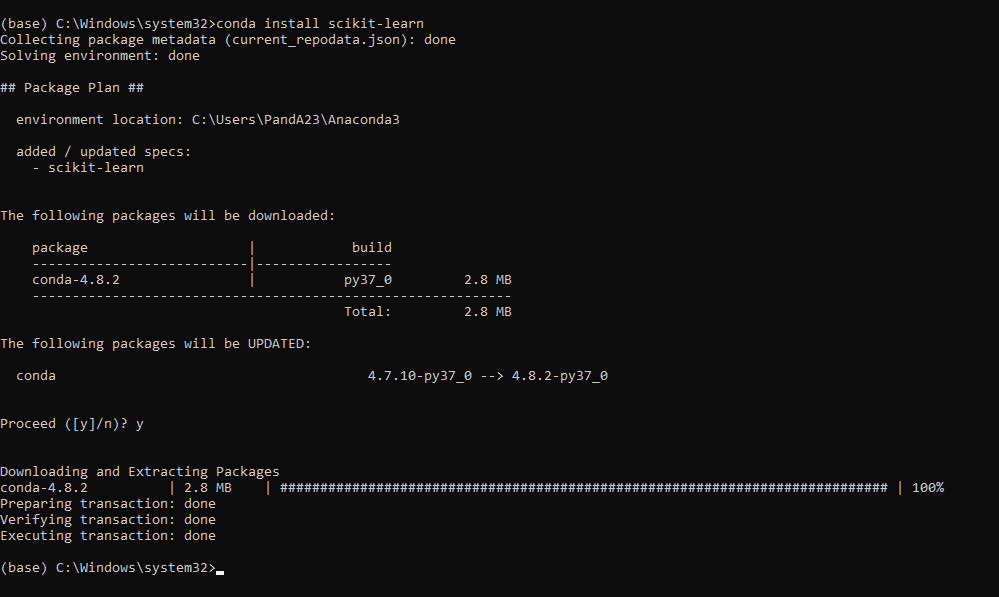
\includegraphics[width=4cm]{figures/1174087/1/instalasi.png}
		\centering
		\caption{Instalasi Package Scikit Learn}
	\end{figure}
	\begin{figure}[H]
		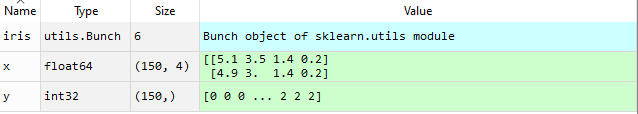
\includegraphics[width=4cm]{figures/1174087/1/variable.png}
		\centering
		\caption{Isi Variabel Explorer}
	\end{figure}
	\item Mencoba loading an example dataset
	\hfill\break
	\lstinputlisting[firstline=8, lastline=12]{src/1174087/1/1174087.py}
	\item Mencoba Learning dan predicting
	\hfill\break
	\lstinputlisting[firstline=14, lastline=24]{src/1174087/1/1174087.py}
	\item Mencoba Model Persistence
	\hfill\break
	\lstinputlisting[firstline=26, lastline=36]{src/1174087/1/1174087.py}
	\item Mencoba Conventions
	\hfill\break
	\lstinputlisting[firstline=38, lastline=50]{src/1174087/1/1174087.py}
\end{enumerate}

\subsection{Penanganan Error}
\begin{enumerate}
	\item ScreenShoot Error
	\begin{figure}[H]
		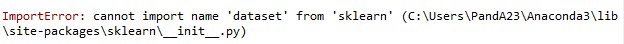
\includegraphics[width=4cm]{figures/1174087/1/import.png}
		\centering
		\caption{Import Error}
	\end{figure}
	
	\item Tuliskan Kode Error dan Jenis Error
	\begin{itemize}
		\item Import Error
	\end{itemize}
	\item Cara Penangan Error
	\begin{itemize}
		\item Import Error
		\hfill\break
		Dengan Menginstall Library Yang Tidak Ditemukan atau Memperperbaiki Penulisan Library 
	
	\end{itemize}
\end{enumerate}

\subsection{Bukti Tidak Plagiat}
\begin{figure}[H]
	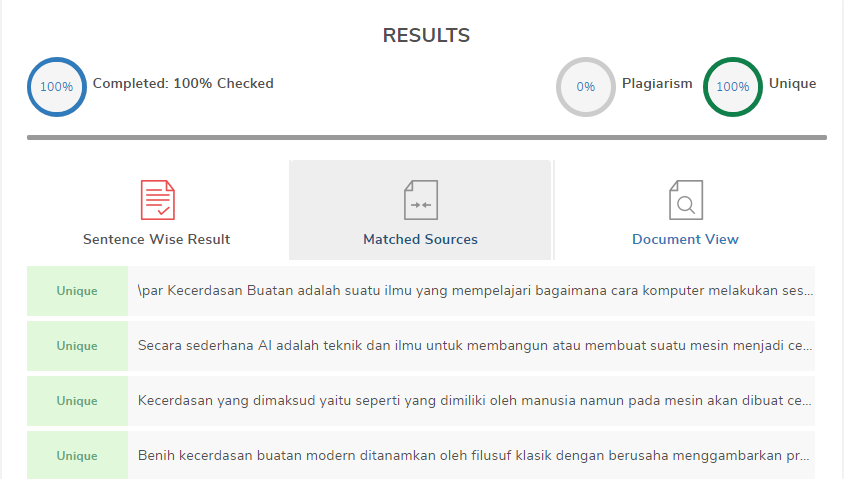
\includegraphics[width=4cm]{figures/1174087/1/plagiat.png}
	\centering
	\caption{Bukti Tidak Melakukan Plagiat}
\end{figure}